%%%%%%%%%%%%%%%%%%%%%%%%%%%%%%%%%%%%%%%%%
% Beamer Presentation
% LaTeX Template
% Version 1.0 (10/11/12)
%
% This template has been downloaded from:
% http://www.LaTeXTemplates.com
%
% License:
% CC BY-NC-SA 3.0 (http://creativecommons.org/licenses/by-nc-sa/3.0/)
%
%%%%%%%%%%%%%%%%%%%%%%%%%%%%%%%%%%%%%%%%%

%----------------------------------------------------------------------------------------
%	PACKAGES AND THEMES
%----------------------------------------------------------------------------------------

\documentclass{beamer}
\usepackage{hyperref}
\usepackage{url}
\usepackage{ulem}
\usepackage{tikz}
\usepackage{multicol}
\usetikzlibrary{fit,calc,positioning,decorations.pathreplacing,matrix}
\usetikzlibrary{positioning}
\mode<presentation> {

% The Beamer class comes with a number of default slide themes
% which change the colors and layouts of slides. Below this is a list
% of all the themes, uncomment each in turn to see what they look like.

%\usetheme{default}
%\usetheme{AnnArbor}
%\usetheme{Antibes}
%\usetheme{Bergen}
%\usetheme{Berkeley}
%\usetheme{Berlin}
%\usetheme{Boadilla}
%\usetheme{CambridgeUS}
%\usetheme{Copenhagen}
%\usetheme{Darmstadt}
%\usetheme{Dresden}
%\usetheme{Frankfurt}
%\usetheme{Goettingen}
%\usetheme{Hannover}
%\usetheme{Ilmenau}
%\usetheme{JuanLesPins}
%\usetheme{Luebeck}
%\usetheme{Madrid}
%\usetheme{Malmoe}
%\usetheme{Marburg}
%\usetheme{Montpellier}
%\usetheme{PaloAlto}
%\usetheme{Pittsburgh}
\usetheme{Rochester}
%\usetheme{Singapore}
%\usetheme{Szeged}
%\usetheme{Warsaw}

% As well as themes, the Beamer class has a number of color themes
% for any slide theme. Uncomment each of these in turn to see how it
% changes the colors of your current slide theme.

%\usecolortheme{albatross}
%\usecolortheme{beaver}
%\usecolortheme{beetle}
%\usecolortheme{crane}
%\usecolortheme{dolphin}
%\usecolortheme{dove}
%\usecolortheme{fly}
%\usecolortheme{lily}
%\usecolortheme{orchid}
%\usecolortheme{rose}
%\usecolortheme{seagull}
%\usecolortheme{seahorse}
%\usecolortheme{whale}
%\usecolortheme{wolverine}

%\setbeamertemplate{footline} % To remove the footer line in all slides uncomment this line
%\setbeamertemplate{footline}[page number] % To replace the footer line in all slides with a simple slide count uncomment this line

%\setbeamertemplate{navigation symbols}{} % To remove the navigation symbols from the bottom of all slides uncomment this line
}

\usepackage{graphicx} % Allows including images
\usepackage{booktabs} % Allows the use of \toprule, \midrule and \bottomrule in tables

%----------------------------------------------------------------------------------------
%	TITLE PAGE
%----------------------------------------------------------------------------------------

\title[Computational Medicine Paper Club]{Discovering robust protein biomarkers for disease from relative expression reversals in 2-D DIGE data \cite{anderson2007discovering}} % The short title appears at the bottom of every slide, the full title is only on the title page

\author{Yanyu Liang} % Your name
\institute[CMU] % Your institution as it will appear on the bottom of every slide, may be shorthand to save space
{
Carnegie Mellon University \\ % Your institution for the title page
\medskip
\textit{yanyul@andrew.cmu.edu} % Your email address
}
\date{\today} % Date, can be changed to a custom date

\begin{document}

\begin{frame}
\titlepage % Print the title page as the first slide
\end{frame}

\begin{frame}
\begin{multicols}{2}
\frametitle{Overview} % Table of contents slide, comment this block out to remove it
\tableofcontents % Throughout your presentation, if you choose to use \section{} and \subsection{} commands, these will automatically be printed on this slide as an overview of your presentation
\end{multicols}
\end{frame}

%----------------------------------------------------------------------------------------
%	PRESENTATION SLIDES
%----------------------------------------------------------------------------------------

%------------------------------------------------
\section{Background} % Sections can be created in order to organize your presentation into discrete blocks, all sections and subsections are automatically printed in the table of contents as an overview of the talk
%------------------------------------------------

\subsection{Proteomics} % A subsection can be created just before a set of slides with a common theme to further break down your presentation into chunks

\begin{frame}
\frametitle{What is Proteomics?}
\begin{columns}[c] % The "c" option specifies centered vertical alignment while the "t" option is used for top vertical alignment
\column{.65\textwidth} % Left column and width
\begin{itemize}
\item Proteomics tells the expression level of \textbf{proteins} in the cell
\item Protein level is important for diagnosis (\textit{e.g.} urinary protein for kidney diseases)
\item Proteomics gives the whole cell proteins' level \textbf{simultaneously}
\item Protein expression vs. Gene expression (DNA microarray)
\end{itemize}
\column{.3\textwidth} % Right column and width
\begin{figure}
\includegraphics[width=0.9\linewidth]{Central_Dogma_of_Molecular_Biochemistry_with_Enzymes.jpg}
\cite{central_dogma}
\end{figure}
\end{columns}
\end{frame}

%------------------------------------------------

\begin{frame}
\frametitle{Proteomics Technology}
\begin{itemize}
\item Mass Spectrometry (only for research now)
\item Electrospherosis (SDS-PAGE, 2D-DIGE\cite{unlu1997difference})
\item 2D electrophoresis: Isoelectric focusing (charge) \& SDS-PAGE (mass)
\item Three samples on one gel in 2D-DIGE
\end{itemize}
\begin{figure}
\includegraphics[width=1\linewidth]{dige.png}
\cite{appliedbiomicsDIGE}
\end{figure}
\end{frame}

%------------------------------------------------
\subsection{Protein Biomarker Discovery} % A subsection can be created just before a set of slides with a common theme to further break down your presentation into chunks
%------------------------------------------------
\begin{frame}
\frametitle{What is Biomarker?}
\begin{itemize}
\item \textit{A biomarker is a \uuline{measurable indicator} of a \uuline{specific biological state}, particularly one relevant to the risk of contraction, the presence or the stage of disease.}\cite{rifai2006protein}
\item Can be used for diagnosis, monitor dieases, select treatment, ...
\item Few of them are used in reality, because to "discover" a robust, reproducible biomarker is hard
\item Find biomarker vs Find classification rule
\end{itemize}
\end{frame}

%------------------------------------------------
\section{Objective} % A subsection can be created just before a set of slides with a common theme to further break down your presentation into chunks
%------------------------------------------------
\begin{frame}
\frametitle{Objective}
\begin{itemize}
\item Find protein biomarker, using 2D-DIGE data
\end{itemize}
\end{frame}

%------------------------------------------------
\section{Challenges}
%------------------------------------------------
%------------------------------------------------
\subsection{Experimental Varibilities}
%------------------------------------------------
\begin{frame}
\frametitle{Reproducibility}
\begin{itemize}
\item Different dyes may lead to different intensity for single spot
\item The result is sensitive to the loading amount 
\item If we use the intensity of the spot directly in gel, we definitely need nomraization:
  \begin{align*}
    X^* = \frac{X - \mu_X}{\sigma_X}
  \end{align*}
\item And there are alternative normalization techniques, like dye swapping
\item But, they generate different results (not robust)
\item It seems normalization always introduces artifact, so we need a "normalization-free" method 
\end{itemize}
\end{frame}

%------------------------------------------------
\subsection{Classifier Interpretability}
%------------------------------------------------
\begin{frame}
\frametitle{Interpretability}
\begin{itemize}
\item Many well-performing classifiers have complicated decision rules which are hard to interpret
\item SVM, LDA, k-NN
\end{itemize}
  \begin{figure}
    \begin{minipage}{.3\textwidth}
      \includegraphics[width=0.9\linewidth]{SVM.png}
      \cite{SVM}
    \end{minipage}
  	\begin{minipage}{.3\textwidth}
      \includegraphics[width=0.9\linewidth]{LDA.png}
      \cite{LDA}
    \end{minipage}
    \begin{minipage}{.3\textwidth}
      \includegraphics[width=0.9\linewidth]{Map5NN.png}
      \cite{kNN}
    \end{minipage}
  \end{figure}
\end{frame}
%------------------------------------------------
\subsection{Technical Replicates}
%------------------------------------------------
\begin{frame}
\frametitle{Handling Technical Replicates}
\begin{itemize}
\item Some samples are not idenpendent, because they are technical replicates
\end{itemize}
\centering
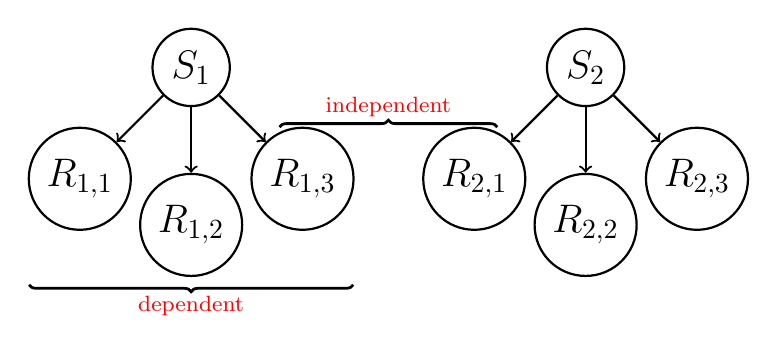
\begin{tikzpicture}[auto, node distance=2cm, every loop/.style={},
                      thick,main node/.style={circle,draw,font=\sffamily\Large\bfseries}]

      \node[main node] (1) {$S_1$};
      \node[main node] (2) [right=4cm of 1] {$S_2$};
      \node[main node] (4) [below left of = 1] {$R_{1, 1}$};
      \node[main node] (5) [below of = 1] {$R_{1, 2}$};
      \node[main node] (6) [below right of = 1] {$R_{1, 3}$};
      \node[main node] (7) [below left of = 2] {$R_{2, 1}$};
      \node[main node] (8) [below of = 2] {$R_{2, 2}$};
      \node[main node] (9) [below right of = 2] {$R_{2, 3}$};

      \draw[->] (1) -- (4);
      \draw[->] (1) -- (5);
      \draw[->] (1) -- (6);
      \draw[->] (2) -- (7);
      \draw[->] (2) -- (8);
      \draw[->] (2) -- (9);

      \draw[decoration={brace,mirror,raise=25pt},decorate,line width=1pt] 
  ([xshift=-5pt]4.south west) -- ([xshift=5pt]6.south east) node [red,midway,yshift=-40pt] {\footnotesize
dependent};
 	  \draw[decoration={brace,raise=32pt},decorate,line width=1pt] 
  ([xshift=5pt]6.south west) -- ([xshift=-5pt]7.south east) node [red,midway,yshift=32pt] {\footnotesize
independent};

\end{tikzpicture}
\end{frame}

\addtocontents{toc}{\newpage}
%------------------------------------------------
\section{RER Algorithm}
%------------------------------------------------
%------------------------------------------------
\subsection{Training (K-)TSP Classifier}
%------------------------------------------------
\begin{frame}[fragile]
\frametitle{(K-)TSP Binary Classifier \cite{geman2004classifying}\cite{tan2005simple}}
Suppose $\mathbf{X}_i = (X_i^{(1)}, X_i^{(2)}, ..., X_i^{(p)})$ and class label is $Y_i$.\\
Define $P^c_{i,j} = \Pr(X^{(i)} > X^{(j)}|Y = c)$, where $c \in \{0, 1\}$.\\
Define $\Delta_{i, j} = |P^0_{i, j} - P^1_{i, j}|$ and $\delta_{i, j} = P^0_{i, j} - P^1_{i, j}$.
\begin{exampleblock}{TSP's Principle}
Select best (K) pair(s) of $i, j$ with top $\Delta_{i, j}$.\\
Classify new sample $\mathbf{X}$:
	\[
	Y = 
	\begin{cases}
	0, \text{if } \text{sign}(\delta_{i, j})(X^{(i)} - X^{(j)}) > 0\\
	1, \text{otherwise} 
	\end{cases}
	\]
\end{exampleblock}
\end{frame}

\begin{frame}
\frametitle{(K-)TSP Binary Classifier \cite{geman2004classifying}\cite{tan2005simple}}
\begin{itemize}
\item In practice, $\hat{P}^c_{i, j} = \frac{\sum\limits_{s \in C} I(X_s^{(i)} > X_s^{(j)})}{|C|}$, where $C = \{\mathbf{X_s}: Y_s = c\}$
\item For K-TSP, K is selected using Leave-One-Out-Cross-Validation
\item Notice that if we assume $\Pr(Y = 0) = \Pr(Y = 1)$, training error is $\frac{1}{2}(1 - \Delta_{i, j})$, which gives us an intuition why choose largest $\Delta_{i, j}$.
\end{itemize}
\end{frame}

\begin{frame}
\frametitle{Properties of TSP Classifier}
\begin{itemize}
\item Easy to perform  
\item Invariant to normalization (Rank based method and normalization is order-preserving)
\item Simple classification rule, only includes a few pairs of proteins (Easy to interpret)
\item No parameter to tune except for k
\end{itemize}
\begin{figure}
  \includegraphics[width=0.8\linewidth]{TSP_example.png}
  \cite{geman2004classifying}
\end{figure}
\end{frame}

%------------------------------------------------
\subsection{Estimiating Error}
%------------------------------------------------
\begin{frame}
\frametitle{Generalization Error}
\begin{itemize}
\item Estimated using LOOCV
\item error rate $= \frac{\text{incorrectly classified}}{\text{total data}}$
\item "Leave One Out" means to leave all technical replicates from the same sample out
\item "Incorrectly classified" means any left replicates are wrongly classified
\item It is more strict than treating all replicates as independent samples
\end{itemize}
\end{frame}

%------------------------------------------------
\subsection{Permutation Analysis}
%------------------------------------------------

\begin{frame}[fragile] % Need to use the fragile option when verbatim is used in the slide
\frametitle{Permutation Analysis}
To answer "How significant is our dicovery based on such dataset?"
\begin{exampleblock}{Permutation Analysis}
\textbf{Step 1} Shuffling the samples' label (not replicates' label)\\
\textbf{Step 2} Measure generalization error\\
\textbf{Repeat 1 and 2}\\
\textbf{Then} Get a distribution of generalization error\\
P-value can be estimated as the frequency that error rate is smaller than the one computed from true labeling
\end{exampleblock}
\end{frame}

%------------------------------------------------
\section{Experimental Details}
%------------------------------------------------
\begin{frame}
\frametitle{Preparing 2D-DIGE data}
\begin{itemize}
\item For each gel, two protein samples are colored by Cy3 and Cy5 respectively
\item Internal standard is prepared as the mixture of all experimental samples, labeled by Cy2
\item Internal standard gives a common position reference for all gels
\item It also gives the background intensity of protein (different proteins have different background intensities)
\item The raw data is the intensity of every spot on the gel
\end{itemize}
\end{frame}

\begin{frame}
\frametitle{Preparing 2D-DIGE data}
\begin{itemize}
\item Number the spot using $p$. To generate $\mathbf{X}$:
\begin{align*}
  X^{(p)} = \frac{\text{Intensity}(p_X)}{\text{Intensity}(p_{Cy2})}
\end{align*}
\item Notice that it is unnormalized data and we can further normalize it using general procedure
\end{itemize}
\end{frame}

%------------------------------------------------
\section{Results}
%------------------------------------------------
\begin{frame}
\frametitle{Cell Samples}
\begin{figure}
\includegraphics[width=0.8\linewidth]{cell.png}
\end{figure}
\begin{itemize}
\item Three types of cells
\item Each type has three samples
\item Each sample has several replicates
\end{itemize}
\end{frame}

\begin{frame}
\frametitle{Gel Layout for Training}
\begin{figure}
\includegraphics[width=0.6\linewidth]{train_layout.png}
\end{figure}
\end{frame}

\begin{frame}
\frametitle{Gel Layout for Validation}
\begin{figure}
\includegraphics[width=0.8\linewidth]{valid_layout.png}
\end{figure}
\end{frame}

\begin{frame}
\frametitle{Classifier Performance}
\begin{figure}
\includegraphics[width=1\linewidth]{results.png}
\end{figure}
\begin{itemize}
\item K-TSP not only works well on normalized data but on unnormalized data (\textit{Raw BVA Ratio})
\end{itemize}
\end{frame}

\begin{frame}
\frametitle{Decision Boundary of K-TSP}
\begin{figure}
  \begin{minipage}{.45\textwidth}
  	\includegraphics[width=.9\linewidth]{db_train.png}
  \end{minipage}
  \begin{minipage}{.45\textwidth}
  	\includegraphics[width=.9\linewidth]{db_valid.png}
  \end{minipage}
\end{figure}
\begin{itemize}
\item K-TSP selects Spot 530 and Spot 786 as pair of spots for classification
\end{itemize}
\end{frame}

\begin{frame}
\frametitle{Significance of Discovery}
\begin{figure}
\includegraphics[width=.5\linewidth]{significance.png}
\end{figure}
\begin{itemize}
\item P-value of the discovery on the training set $<$ 0.022
\end{itemize}
\end{frame}

\begin{frame}
\frametitle{Determining the Proteins at the Spots}
\begin{itemize}
\item Mass Spectrometry is used to find which protein is at the selected spot
\item Spot 530 is Enolase 1 [Homo sapiens] (NCBI accession number is gi13323287)
\item Spot 768 is Tropomyosin isoform 3/4 [Homo sapiens] (NCBI accession number is gi54696136/55665781)
\end{itemize}
\end{frame}

%------------------------------------------------
\section{Discussion}
%------------------------------------------------
\begin{frame}
\frametitle{Advantages}
\begin{itemize}
\item Normalization-free, avoid to introduce artifact
\item Easy to make use of data from different resources (done by different labs and protocols)
\end{itemize}
\end{frame}

\begin{frame}
\frametitle{Drawbacks}
\begin{itemize}
\item Fairly small datasets
\item Does not take PTMs into consideration
\item Limited decision boundary that may fail in some cases
\item To maximize $\Delta_{i, j}$ is not valid when marginals are not equal
\end{itemize}
\end{frame}

\begin{frame}
\frametitle{Improvements}
\begin{columns}[c] % The "c" option specifies centered vertical alignment while the "t" option is used for top vertical alignment
\column{.6\textwidth} % Left column and width
\begin{itemize}
\item $\Pr(\frac{X^{(i)}}{X^{(j)}} > 1) \Rightarrow \Pr(\frac{X^{(i)}}{X^{(j)}} > k)$ ? 
\item For more difficult dataset, boosting of TSP might be a choice comparing to K-TSP ?
\item If marginals of class labels are not equally distributed, minimizing $\Pr(c = 0)(1 - P^0_{i, j}) + \Pr(c = 1)P^1_{i, j}$ is more reasonable than maximizing $\Delta_{i, j}$ ?
\end{itemize}
\column{.4\textwidth} % Left column and width
\begin{figure}
  \includegraphics[width=1\linewidth]{improve.png}
\end{figure}
\end{columns}
\end{frame}

%------------------------------------------------
\begin{frame}[allowframebreaks]
\frametitle{References}
\footnotesize
\bibliography{my_ref} 
\bibliographystyle{IEEEtran}
\end{frame}

%------------------------------------------------

\begin{frame}
\Huge{\centerline{The End}}
\end{frame}

%----------------------------------------------------------------------------------------

\end{document} 